% Calibrating the panels
\section{Further studies on the Cosmic Ray Tracker}

Using the software bundled with the \gls{feb} and CalibRaTe, 3 further sets of observations are made to analyse the behaviour of the \gls{crt} modules, test the functionality of the data acquisition software and show the versatility of the evaluation tools.
This section lists the observations made with the \gls{crt} modules and analyzes part of the data of the observation sets.

\subsection{Sets of observations}

The \gls{feb}'s power supply voltage affects the generation of the bias voltage $V_\text{bias}$ and the output of the discriminator used to determine the threshold.
A change in the power supply voltage will changes the visible spectrum in the histograms.
Several sets of measurements have been taken using different power supply voltages to see this behavior and other effects.
The set of parameters for these observations are listed in table \ref{tab:os1}.

\begin{table}
  \centering
  \begin{tabular}{ c c c }
    Date       & \gls{feb} \& panels & Power supply voltage [V] \\
    \toprule
    2016-07-30
      & & \begin{tabular}{c c c c c}
        4.50 & 4.60 & 4.70 & \ldots & 5.10 \\
      \end{tabular}
    \\
    2016-08-03 & (71, 371) & 5.20   \\
    2016-08-04 &
      & \begin{tabular}{c c c}
        5.30 & 5.40 & 5.50 \\
      \end{tabular}
    \\
    \bottomrule
    \\
  \end{tabular}
  \caption{%
    Parameters of the observation set OS1.
    The \gls{feb} was powered with a Gw Instek GPS-4304 Power Supply, the power supply voltage's value was set manually and checked with a Fluke 115 Multimeter with an uncertainty of 0.01V.
    The power supply displayed a constant current at 0.52 (0.01) A.
  }
  \label{tab:os1}
\end{table}

The used data acquisition software was written to read data from several modules in parallel.
Another feature of the software is to permit the acquisition of data for a set of \gls{dac} settings without human interaction.
To test this functionality, the set of observations OS2 -- listed in table \ref{tab:os2} was made.

\begin{table}
  \centering
  \begin{tabular}{ c c c }
    Date       & \glspl{feb} \& panels & \gls{dac} setting [bin] \\
    \toprule
    2016-08-07
      & \begin{tabular}{ c c }
        (75, 375) & (76, 376) \\
        (77, 377) & (78, 378) \\
        (79, 379) & (80, 380) \\
      \end{tabular}
      & \begin{tabular}{ c c c c c }
         180 & 181 & 182 & \ldots & 200 \\
      \end{tabular}
    \\
    \bottomrule
    \\
  \end{tabular}
  \caption{%
    Parameters of the observation set OS2.
    The \gls{feb} was powered with rack power supply, the power supply voltage was kept constant at 4.63 (1) V and checked with a Fluke 115 Multimeter.
  }
  \label{tab:os2}
\end{table}

\subsection{Effects of changing power supply voltages on the pedestal}

A gaussian distribution is fitted around the pedestal of every \gls{sipm} for every parameter of observation set OS1.
The resulting positions, width and amplitudes are plotted in dependency of the power supply voltage in figure \ref{fig:pedestal_input}.

\begin{figure*}
  \centering
  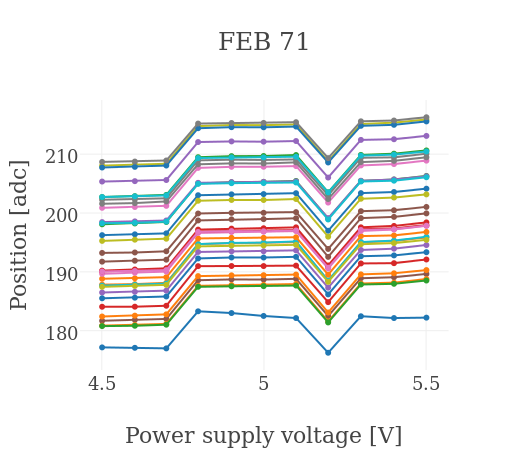
\includegraphics[width=.32\textwidth]{studies/input_voltages/pedestal_position_narrow}
  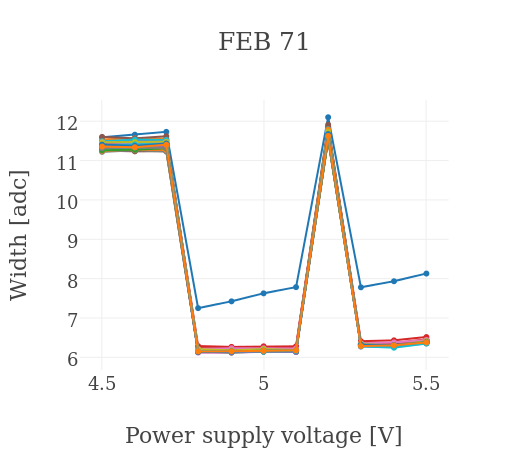
\includegraphics[width=.32\textwidth]{studies/input_voltages/pedestal_width_narrow}
  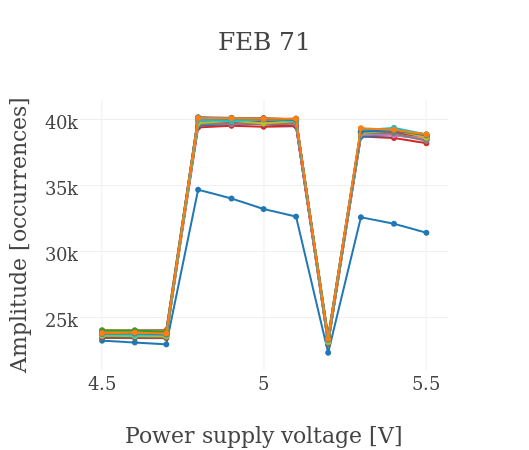
\includegraphics[width=.32\textwidth]{studies/input_voltages/pedestal_amplitude_narrow}
  \caption{
    Fitted pedestal positions for the 32 \glspl{sipm} of observation set OS1.
    Every colored line represents a \gls{sipm} of the \gls{crt} module.
    The uncertainties of the fits are tiny and not displayed in the plot.
  }
  \label{fig:pedestal_input}
\end{figure*}

The correlation of the signal of the 32 \glspl{sipm} is evident.
The plot also shows, that the pedestal of the \gls{crt} module has at least two diferent 'regimes'.
Notice the change of all three parameters at power supply voltages at and around 4.7V and 5.1V.
The pedestal changes by $\approx10\%$, while the width and amplitude change by a factor of 2.
The reason for this behaviour requires further study.

\subsection{Influences of the power supply voltage on the spectrum}

The behaviour of the spectrum is observed for changing power supply voltages, using the data from set OS1.
The spectrum of a \gls{sipm} is is displayed in dependency of the power supply voltage in figure \ref{fig:spectrum_input}.
\begin{figure}
  \centering
  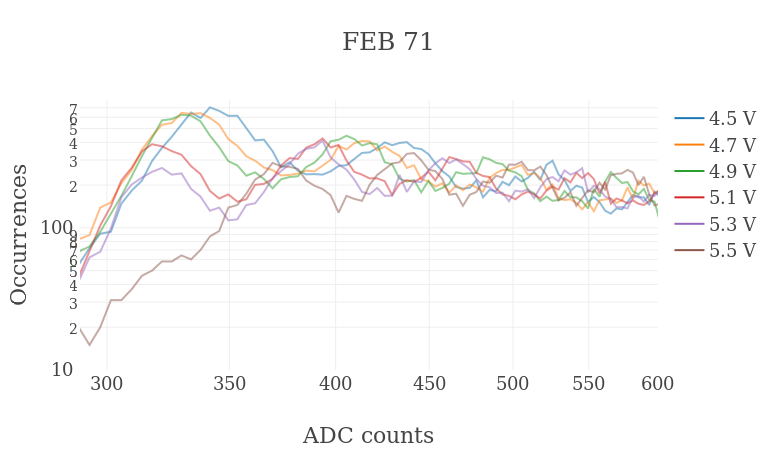
\includegraphics[width=\textwidth]{studies/input_voltages/spectrum_cutout}
  \caption{%
    Observed spectrum for changing power supply voltages.
    A shift of the spectrum to the left is clearly visible with increasing power supply voltage.
  }
  \label{fig:spectrum_input}
\end{figure}

The figure shows the spectrum of a \gls{sipm} for varying power supply voltages.
It is clearly visible, that the spectrum depends on the power supply voltage.
It is not obvious, though expected, that the distance between peaks change.
The shift of the spectrum to the left with raising voltage is undeniable.
This behavior shows the importance of a stable power supply voltage.

\subsection{Event rate vs. power supply voltages}

During \gls{daq} an important change of the time spent to acquire the same amount of data was noticed.
To study this behavior further, the \gls{feb}'s event rates were observed and stored using the output of the monitoring software febmon.
Since febmon does not specify which \gls{sipm} originates the observed event rate, spectra of the event rates are generated.
The event rate spectrum for every voltage is plotted histogram \ref{fig:eventrate_input}.

\begin{figure}
  \centering
  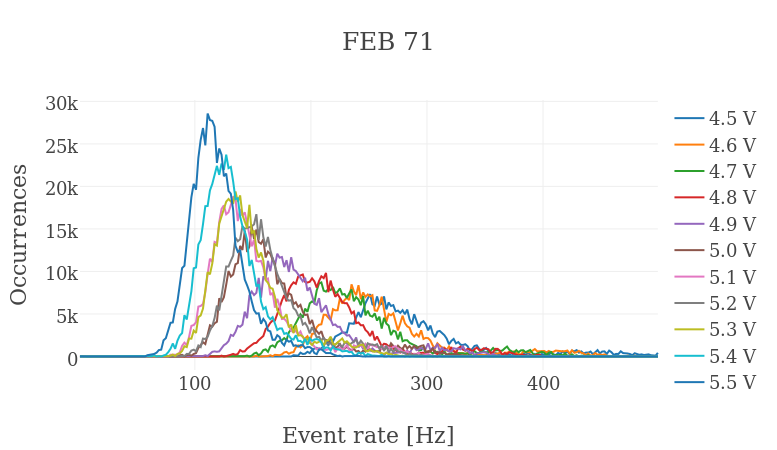
\includegraphics[width=\textwidth]{studies/input_voltages/event_rates}
  \caption{%
    Observed spectra of the event rates for \gls{feb} 71 and panel 371 for different power supply voltages.
    The shift to the left with increasing power supply voltage is evident.
  }
  \label{fig:eventrate_input}
\end{figure}

\pagebreak
The plot shows gaussian distributed spectra, whose shape and position depend cleary on the power supply voltage.
The distribution shifts to the left with increasing power supply voltage while getting thinner and gaining amplitude.

To see this effect more clearly, a gaussian distribution is fitted to each spectrum to determine its amplitude, position and width.
These fit parameters are plotted in dependence of the power supply voltage in figure \ref{fig:eventrate2_input} to see the dependency on the power supply voltage.

\begin{figure*}
  \centering
  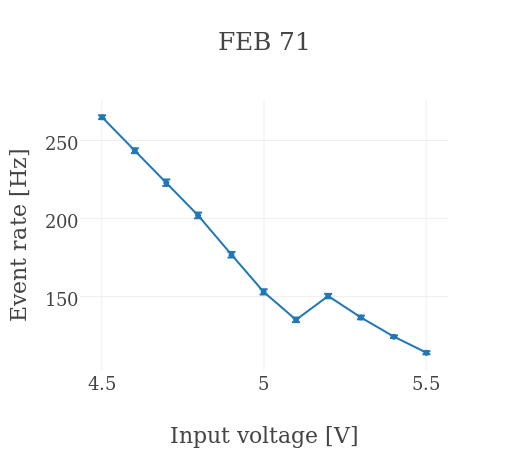
\includegraphics[width=.325\textwidth]{studies/input_voltages/eventrate_vs_voltage}
  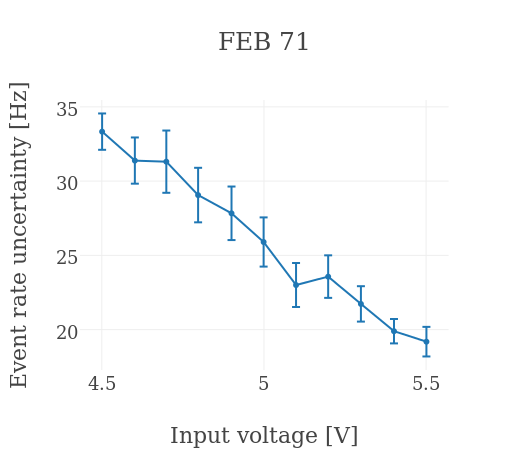
\includegraphics[width=.325\textwidth]{studies/input_voltages/eventrate_uncertainty_vs_voltage}
  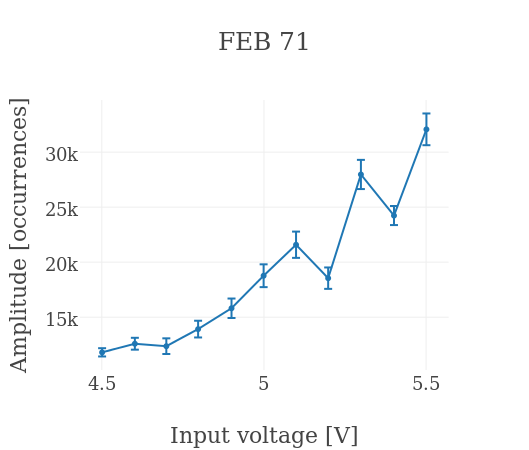
\includegraphics[width=.325\textwidth]{studies/input_voltages/eventrate_amplitude_vs_voltage}
  \caption{Fit parameters (fltr: position, width and amplitude) of the event rate distributions in dependency of the power supply voltages.}
  \label{fig:eventrate2_input}
\end{figure*}

The decrease of the event rate with increasing power supply voltage is obvious.
This decrease suggests a change in the detection efficiency.
The dispersion of the event rate spectra within a \gls{crt} module decreases with higher voltage, consequently the amplitude of the gaussians increases with higher power supply voltage.
Since the event rates decrease with higher voltage and each set of measurements contains the same amount of events, the time febmon observed the event rate increased.
Due to febmon's constant observation rate, the number of observations and therefore the amplitude of the spectra increases with longer observation time.

\subsection{Effects of changing bias voltages on the pedestal}

Since the pedestal is an indicator of the noise in the signal, studying its behavior in dependency of the bias voltage is of importance.
For this reason the pedestal is studied for the observation set OS2.
The positions and widths of the fitted gaussians are displayed in figures \ref{fig:pedestal_pos_bias} and \ref{fig:pedestal_wid_bias}.

\begin{figure}
  \centering
  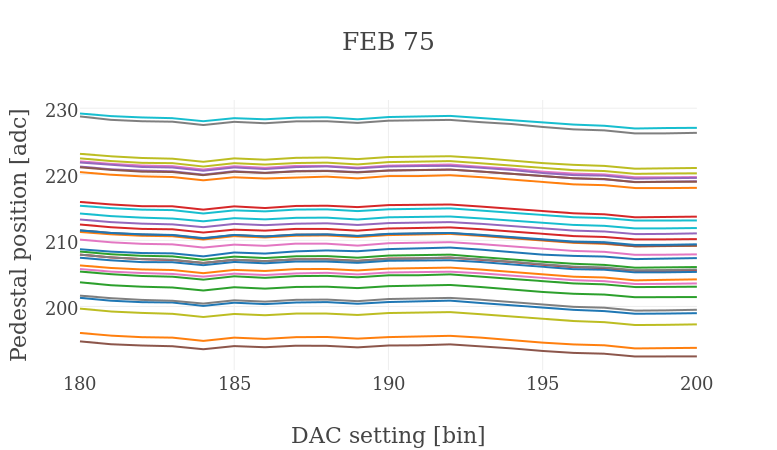
\includegraphics[width=\textwidth]{studies/bias_voltages/pedestal_position_75}
  \caption{%
    Fitted pedestal positions in dependency of the bias voltage for one of the \gls{feb} of a observation set OS2.
    Every colored line represents a \gls{sipm} of the module.
  }
  \label{fig:pedestal_pos_bias}
\end{figure}

The plot displays a clear correlation of the pedestals change in position for all the \gls{sipm} signals.
This correlation indicates the independency of the \gls{sipm} on the change of position, suggesting the \gls{feb} as main contributor to this parameter.
This correlation is visible for all observed \gls{crt} panels.
The positions of the pedestals depend on the \gls{sipm}.
The spread of pedestal positions is assumed to be related to the spread of gains of an uncalibrated \gls{crt} module.

\begin{figure}
  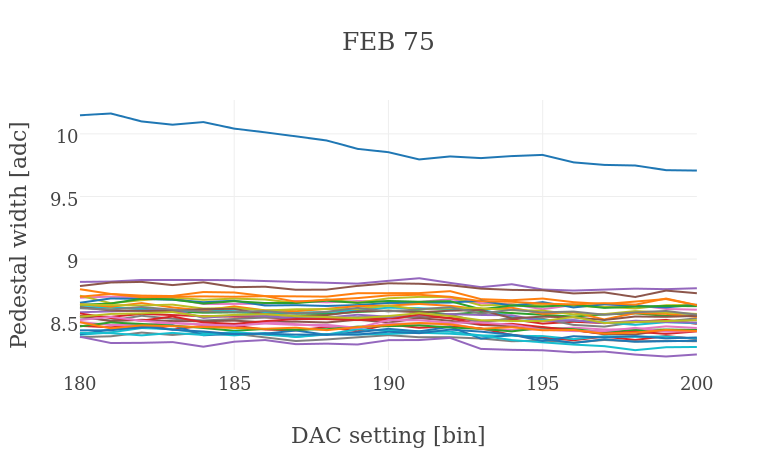
\includegraphics[width=\textwidth]{studies/bias_voltages/pedestal_position_uncertainty_75}
  \caption{%
    Fitted pedestal widths in dependency of the bias voltage for one of the \gls{feb} of a observation set OS2.
    The widths of the pedestals are similar to each other, only one of the \glspl{sipm} has a wider pedestal.
    Every colored line represents a \gls{sipm} of the module.
  }
  \label{fig:pedestal_wid_bias}
\end{figure}

The width of the pedestal is similar for all the \glspl{sipm} of the same \gls{crt} module.
Only one \gls{sipm}'s pedestal is considerably wider than the rest.
This behavior is attributed to the greater difference in voltage during digitazing process for thefirst \gls{sipm} which leads to a greater uncertainty of the \gls{adc}'s input.
The width of the first \gls{sipm}'s pedestal tends to decrease with increasing bias voltage.

The computed positions and widths of the pedestal are counted for all the sets of OS2 and displayed in figure \ref{fig:pedestal_pos_spectra_bias}.

\begin{figure}
  \centering
  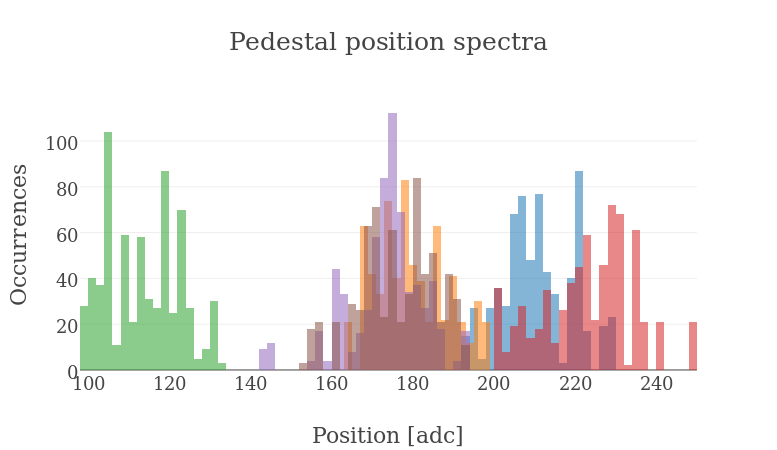
\includegraphics[width=\textwidth]{studies/bias_voltages/pedestal_position_spectra}
  \caption{
    The spectra of the fitted positions of the pedestal for the observation set OS2.
    Every color represents a different \gls{crt} module.
  }
  \label{fig:pedestal_pos_spectra_bias}
\end{figure}

The pedestals are distributed around a mean value which varies from \gls{crt} module to \gls{crt} module.
The distribution of the pedestals give an idea of the variation of the pedestal.

\begin{figure}
  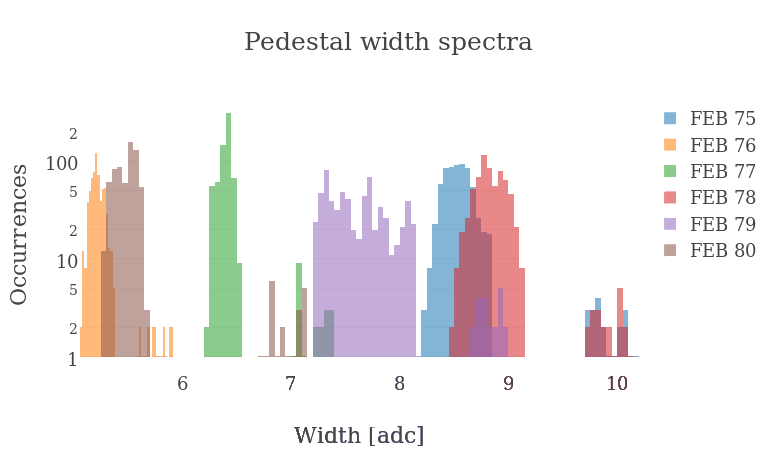
\includegraphics[width=\textwidth]{studies/bias_voltages/pedestal_width_spectra}
  \caption{
    The spectra of the fitted widths of the pedestal for the observation set OS2.
    Each distribution contains the computed widths of all the \glspl{sipm} for all set bias voltages.
    Each color represents a different \gls{crt} module.
    A feature on the right of every distribution is visible, attributed to the first \gls{sipm} of every \gls{crt} module.
  }
  \label{fig:pedestal_wid_spectra_bias}
\end{figure}

The figure displays a variety of distributions, whose mean and standard deviation depends heavily on the observed \gls{crt} module.
The difference of the first \gls{sipm}'s pedestal width is visible in each distribution.

The change of position and width of the pedestal is observed in dependency of the bias voltage, by computing and counting all the changes of the respective parameters.
The resulting distributions are displayed in figure \ref{fig:pedestal_changes_bias}.

\begin{figure*}
  \centering
  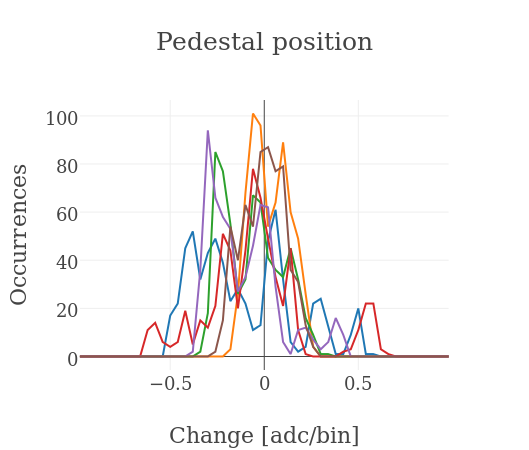
\includegraphics[width=.48\textwidth]{studies/bias_voltages/change_pedestal_position}
  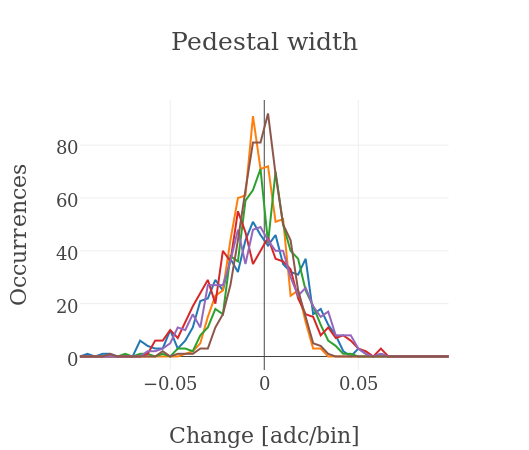
\includegraphics[width=.48\textwidth]{studies/bias_voltages/change_pedestal_width}
  \caption{%
    Histograms displaying the spectrum of changes in pedestal position, width and amplitude for observation set OS2.
  }
  \label{fig:pedestal_changes_bias}
\end{figure*}

The computed spectra of the parameters' differences are distributed around the origin.
The spectra of the pedestals' position is more spread than the spectra of the pedestals' width.

This study is done for a fixed power supply voltage.
Since the power supply voltage incluences the regime of the pedestal, a study including the variation of the power supply voltage and the bias voltage is recommended.
